\documentclass[a4paper]{article}

\usepackage[utf8]{inputenc}
\usepackage[T1]{fontenc}
\usepackage[english,serbian]{babel}
\usepackage{etoolbox}
\usepackage{graphicx}
\usepackage[acronym]{glossaries}

\usepackage[unicode]{hyperref}
\hypersetup{colorlinks,citecolor=green,filecolor=green,linkcolor=blue,urlcolor=blue}

\newacronym{hr}{HR}{Human Resources}
\newacronym{it}{IT}{Information Technology}
\makenoidxglossaries

\newcommand{\quotes}[1]{„#1“}

\begin{document}
    \title{Mobing u programerskom svetu\\ \small{Seminarski rad u okviru kursa\\Metodologija stručnog i naučnog rada\\ Matematički fakultet}}

    \author{Branko Cvetković, Tamara Đukić,\\Dušan Trtica, Petar Đorđević\\branecvele@gmail.com, tamarazdjukic@gmail.com,\\trle83@gmail.com, petar.djordjevic@matf.bg.ac.rs}

    \date{22.~novembar 2023.}

    \maketitle

    \abstract{Mobing je pojava koja se sve češće javlja u poslovnom svetu. Mobing može na različite načine da se ispolji na pojedinca ili grupu ljudi. Takođe može da ostavi manje ili veće posledice na psihu ljudi. U ovom radu ćemo predstaviti mobing kao pojavu i njegove oblike. Zatim ćemo se osvrnuti na posledice mobinga i njegov uticaj na žrtve, kao i na posledice koje mobing ostavlja na kompanije, kao i na načine kojima se može zaštititi od mobinga. Nakon toga ćemo predstaviti i podatke vezane za mobing u Srbiji, ali i u svetu, i završiti primerima mobinga u svetu programiranja.}

    \tableofcontents
    
    %Tamara Đukić
    \newpage
    \section{Uvod}
        Mobing (eng. mobbing) podrazumeva psihičko ili fizičko uznemiravanje pojedinca ili grupe ljudi iz raznih razloga. Najčešće metode uznemiravanja su: ponižavanje, vređanje, ismejavanje, izolovanje iz grupe ljudi, i još mnogo drugih metoda.
        
        Sve ove metode može da vrši jedna osoba ili grupa ljudi na jednu ili više osoba, a najčešći razlog za to je isključivanje iz radne zajednice. Ovakva ponašanja mogu da dovedu do opasnih posledica, fizičkih ili psihičkih, kod pojedinca tokom celog života.
        
        Pojam mobinga nije novi fenomen.\hspace{0.1cm}On je prisutan još iz davnina, od kad postoji ljudski rod, jer se od tad javlja želja za prevladom nad određenima.
        
        Termin \quotes{mobbing} najčešće se koristi u Švedskoj, Nemačkoj i Italiji dok u zemljama engleskog govornog područja nailazimo na termin \quotes{bullying}, a u SAD-u najčešće termin \quotes{work abuse}. Reč \quotes{mobbing} dolazi od engleskog glagola \quotes{to mob} što u prevodu znači bučno navaliti, nasrnuti \cite{stajemobing}.
        
        Prvi naučnik koji je počeo istraživanje ovog fenomena bio je nemački psiholog Heinz Leyman.\hspace{0.1cm}On 1990. godine u \quotes{Mobingu} navodi da je mobing \quotes{komunikativna situacija koja preti da izazove ozbiljnu fizičku i psihičku štetu pojedincu}. Po Lajmanu, svaki radnik tokom svog radnog veka ima 25\% šansi da bude barem jednom žrtva mobinga \cite{leymannmobbing}.
        
    %Petar Đorđević
    \subsection{Kada se javlja mobing?}
        Ako razmatramo povode ili uzroke mobinga, važno je razumeti da su različite situacije i faktori koji mogu doprineti pojavi mobinga na radnom mestu.
        U potencijalne povode za mobing uključeni su \cite{ELCI2014455, ERGIN2023115595, ERTURK20143669, VARAHORNA2023e21096}:
        \begin{itemize}
            \item \textbf{\textit{Konflikti interesa}} - Ljubomora i konflikti interesa, kao što su različiti finansijski ili profesionalni ciljevi, mogu generisati neprijateljsko ponašanje na radnom mestu. Ova dinamika često podstiče zlostavljanje kako bi se postigla dominacija ili eliminisala konkurencija u programerskim firmama.
            \item \textbf{\textit{Neravnoteža moći}} - Kada postoji previše izražena hijerarhija ili neravnoteža moći u organizaciji, može doći do zloupotrebe te moći. Osobe koje zloupotrebljavaju svoj položaj ili autoritet mogu vršiti mobing nad onima koji su pod njihovom kontrolom.
            \item \textbf{\textit{Nedostatak podrške u organizaciji}} - Ako organizacija ne pridaje dovoljno pažnje stvaranju pozitivnog radnog okruženja, nedostatak podrške i nedostatak efikasnih mehanizama rešavanja konflikata mogu doprineti pojavi mobinga.
            \item \textbf{\textit{Stresan posao}} - Teški uslovi rada i visok nivo stresa na poslu mogu predstavljati povod za mobing. Kada zaposleni doživljavaju intenzivan stres ili se suočavaju sa zahtevnim radnim uslovima, to može doprineti tenziji među kolegama. Stresni okviri često stvaraju okolinu u kojoj se radnici osećaju nemoćno, što može olakšati pojavu mobinga kao načina izražavanja frustracija ili oslobađanja napetosti.
            \item \textbf{\textit{Diskriminacija i predrasude}} - Mobing može proisteći iz diskriminacije na osnovu različitih faktora kao što su pol, rasna ili etnička pripadnost, seksualna orijentacija, religija i druge lične karakteristike. Ponašanje zasnovano na predrasudama može dovesti do sistematskog uznemiravanja. Kada organizacija ne promoviše raznolikost i inkluzivnost, to može stvoriti atmosferu u kojoj se određeni pojedinci ili grupe osećaju izolovano ili diskriminisano, što može dovesti do pojave mobinga.
            \item \textbf{\textit{Stilovi upravljanja}} - Loši stilovi upravljanja, poput autoritarnog, ili nedostatka komunikacije, mogu stvoriti neprijateljsko okruženje. Nedostatak jasnih očekivanja i loše komunikacije može doprineti tenzijama i konfliktima. Ako organizacija implicitno ili eksplicitno nagrađuje agresivno ponašanje ili dominaciju nad kolegama, to može stvoriti atmosferu u kojoj se mobing toleriše ili čak promoviše.
            \item \textbf{\textit{Atmosfera straha}} - Kada se u organizaciji uspostavi atmosfera straha, zaposleni postaju potencijalne žrtve mobinga. Strah od gubitka posla, stigmatizacije ili negativnih posledica može podsticati zlostavljanje.
            \item \textbf{\textit{Nedostatak svesti o mobingu}} - U nekim slučajevima, nedostatak svesti o štetnim efektima mobinga može dovesti do tolerancije ili ignorisanja ovakvog ponašanja. Kada zaposleni nisu svesni šta podrazumeva mobing ili kako prepoznati i reagovati na takvo ponašanje, to može doprineti produžavanju problema.
        \end{itemize}
        Sve ove dinamike ukazuju na to da se mobing ne javlja izolovano, već je često rezultat kombinacije različitih faktora.
        Prevencija mobinga stoga zahteva holistički pristup, koji uključuje uspostavljanje jasnih pravila, podršku liderstva, razvoj pozitivne organizacione kulture i edukaciju zaposlenih o štetnim posledicama mobinga. Analiziranje ovih aspekata može pomoći u razumevanju kako i zašto se mobing javlja, pružajući osnovu za razvoj efikasnih strategija prevencije i rešavanja ovakvih problema.
    
        %Tamara Đukić
    \subsection{Vrste mobinga}
        Prema različitim faktorima, mobing se može podeliti na dve glavne grupe \cite{vrstemobinga}:
        \begin{itemize}
            \item \textbf{\textit{Horizontalni}} - javlja se između radnika koji su na istom nivou u hijerarhiji. Često jedna ili više osoba sprovode neku vrstu mobinga na jednu osobu, sa različitim ciljevima: da osoba napusti posao, da bi osobe dobile veću poziciju ili da se pokažu da su emocionalno snažnije.
            \item \textbf{\textit{Vertikalni}} - javlja se između osoba na različitim nivoima hijerarhije. Ovde u većini slučajeva pretpostavljeni vrši mobing nad radnikom, kao i obrnuto.
        \end{itemize}
        
        Postoje i 2 podgrupe mobinga:
        \begin{itemize}
            \item \textbf{\textit{Strateški}} - vezuje se za dogovor upravljačke garniture o potrebi racionalizacije i udaljavanja jednog broja radnika. Stalnim primedbama, ponižavanjima, kažnjavanjima \quotes{izluđuju} zaposlene što podstiče njihov odlazak.
            \item \textbf{\textit{Afektivni ili emotivni}} - odvija se na ličnom nivou (javlja se kao posledica straha od gubitka posla, zbog zavisti i zlobe). Nesposobni radnici svoju nesposobnost kriju spletkarenjem i podmićivanjem svojih kolega na poslu.
            \item Postoji i \textbf{\textit{\quotes{Serijski mobing}}} - kada jedna osoba po odabiru \quotes{uništava} jednog po jednog zaposlenog, a to za posledicu ima \quotes{sekundarni mobing} koji se ogleda u posebnom psihičkom stanju ostalih zaposlenih koji bez uspeha pokušavaju da izađu na kraj sa serijskim mobingom.
        \end{itemize}
        
    \subsection{Specifična ponašanja mobinga}
        Lajman je 1990. godine kroz 300 intervjua prošao 46 specifičnih ponašanja koje zlostavljači koriste protiv svojih žrtava. On je klasifikovao ova ponašanja u pet kategorija \cite{CORNOIU2013708}:
        \begin{itemize}
            \item Radnje koje mogu blokirati izražavanje žrtve - osoba ne može da izrazi svoje stavove pred svojim šefom, prekida se u govoru, ne sme da podržava svoje gledište, zlonamerne primedbe su napravljene protiv nje, vređaju ga, kritikuju, kako profesionalno, tako i na ličnom nivou.
            \item Radnje za izolaciju žrtve - prestupnici nikad ne razgovaraju sa žrtvom ili ako žrtva pokuša da započne razgovor, odgovaraju jednosložno, neprijateljski, ignoriše se fizičko prisustvo žrtve.
            \item Postupci nepoštovanja suda prema žrtvi - protiv žrtve se govore razne glasine o njoj, ismevaju se i smatraju mentalno bolesnim, politička ili verska uverenja žrtve su napadnuti, šale se na račun porekla.
            \item Profesionalna diskreditacija žrtve - žrtvi se ne dodeljuju zadaci ili su dodeljeni zadaci iznad ili ispod njene kvalifikacije, neki od njih su nepotrebni ili apsurdni.
            \item Radnje za ugrožavanje zdravlja žrtve - žrtvi su dodeljeni poslovi koji su opasni ili štetni za njeno zdravlje, pretnja fizičkim nasiljem, laka fizička agresija kao opomena, ozbiljan fizički napad.
        \end{itemize}
        
    \section{Faze mobinga}
    Drugi veliki istaživač fenomena mobinga je Harald Ege. Po Egeu, Lajmanov model se najviše može primeniti na skandinavsko područje, ali se ne odnosi na ostale zemlje. Ege je istaživao ovaj fenomen u Italiji, i definisao 6 faza mobinga \cite{ege2000mobbing}:
    \begin{enumerate}
        \item Nulta faza - Smatra se pred-fazom. U ovoj fazi nema želje za uništavanjem, već ima potrebu biti superioran u odnosu na druge.
        \item Prva faza - \textbf{usmerena na sukob}. U ovoj fazi identifikuje se žrtva, i sukob je usmeren ka toj osobi. Cilj agresora je da ukloni, uništi pojedinca. Takođe, agresor se fokusira i na privatne stvari pojedinca.
        \item Druga faza - \textbf{pojava mobinga}. Napadi još ne izazivaju psihičke simptome ili bolest žrtve, ali stvara se nelagoda, anksioznost, bes.
        \item Treća faza - \textbf{prvi psihički simptomi}. Žrtva počinje da pokazuje neke zdravstvene probleme koji se mogu odužiti na dug vremenski period. Uobičajeni simptomi su: nesanica i problemi sa varenjem.
        \item Četvrta faza - \textbf{greške i zloupotrebe u upravljanju ljudskim resursima}. Mobing postaje javan i često je podstaknut greškama u proceni osoba odeljenja. Prethodna faza dovodi do bolesti žrtve, a učestalost bolesti dovodi do sumnjičavosti kolega.
        \item Peta faza - \textbf{pogoršanje psihofizičkog stanja pojedinca}. Stanje pojedinca se znatno pogoršava. Pojavljuje se blaga ili teška depresija.
        \item Šesta faza - \textbf{isključenje sa posla}. Poslednja faza u kojoj se osoba udaljava sa posla, samoinicijativno ili dobija otkaz usled razvijenih psihičkih problema. 
    \end{enumerate}

    %Petar Đorđević
    \section{Posledice mobinga}
        Mobing predstavlja ozbiljno narušavanje radnog okruženja, stvarajući klimu neprijateljstva i stresa.
        U ovom kontekstu, osim što direktno utiče na psihičko i fizičko zdravlje zaposlenih, mobing ima značajne implikacije i na efikasnost rada organizacije kao celine.
        Pojavom mobinga na radnom mestu otvaraju se vrata nizu ozbiljnih posledica koje se prožimaju kako na pojedinca izloženog agresivnom ponašanju, tako i na samu organizaciju.
    \subsection{Posledice po pojedinca}
        Zaposleni koji se suočavaju sa mobingom na radnom mestu doživljavaju duboke i raznovrsne posledice koje direktno utiču na njihovo fizičko i psihičko stanje \cite{leymannmobbing}.

        Emocionalni teret je jedan od ključnih aspekata, gde žrtve mobinga često iskuse anksioznost, intenzivan emocionalni stres i smanjenje samopouzdanja.
        Povećana izloženost mobingu na radnom mestu često vodi ozbiljnim posledicama za mentalno zdravlje zaposlenih.
        Depresija, osećaj izolacije i gubitak samopouzdanja, česti pratioci mobinga \cite{leymannmobbing}, mogu predstavljati značajan rizik za pojave kao što je povećan rizik suicida \cite{ERGIN2023115595}.
        Ova ozbiljna posledica naglašava potrebu za hitnim prepoznavanjem i efikasnim merama podrške kako bi se zaštitilo mentalno stanje zaposlenih.

        Fizičko zdravlje zaposlenih takođe trpi pod stalnim stresom izazvanim mobingom \cite{CELEP20124761}.
        Neki od fizičkih simptoma koji se javljaju su prehlada, glavobolje, problemi sa snom, čirevi, visok krvni pritisak, bolovi u mišićima, prekomerna konzumacija cigareta i alkohola i drugi.
        
        Socijalna izolacija je česta posledica mobinga \cite{leymannmobbing}. Osećaj stigmatizacije često rezultuje udaljavanjem od kolega, stvarajući okruženje gde je podrška i razumevanje retko prisutno. Žrtve mobinga često izostaju s posla, podnose otkaze ili napuštaju radno mesto zbog nepovoljnih uslova koje stvara toksično radno okruženje.
        
        Smanjenje radne motivacije predstavlja još jedan izazov. Neprijateljsko radno okruženje, karakteristično za mobing, dovodi do gubitka interesovanja za posao i smanjenja radne angažovanosti.
    \subsection{Posledice po firmu}
        Neprijateljsko radno okruženje uzrokovano mobingom može značajno naštetiti samoj organizaciji,
        stvarajući brojne izazove koji se reflektuju na dugoročni uspeh i integritet.

        Razaranje timskog duha i smanjenje produktivnosti postaju očigledni u okruženju punom straha i stresa koji uzrokuje mobing.
        Neprijateljsko radno okruženje otežava efikasnu saradnju između zaposlenih, smanjujući radnu produktivnost i otežavajući ostvarivanje poslovnih ciljeva.
        Smanjeno poverenje u menadžment i firmu dodatno pojačava ovu dinamiku, stvarajući atmosferu nesigurnosti i ograničavajući sposobnost organizacije da zadrži talentovane zaposlene.
        Ova kombinacija faktora može dugoročno ugroziti harmoniju u radnoj sredini i usmeriti organizaciju ka izazovima u održavanju stabilnosti i konkurentske prednosti na tržištu.
        
        Oštećenje ugleda firme je jedna takva ozbiljna posledica.
        Ignorisanje problema mobinga može dovesti do toga da se organizacija doživljava kao nepoželjni poslodavac, što može odbiti potencijalne talente i klijente.
        Reputacija jedne firme često igra ključnu ulogu u njenom dugoročnom uspehu na tržištu.

        Mobing na radnom mestu često uzrokuje povećani odlazak zaposlenih, stvarajući visok obrt radne snage \cite{ELCI2014455}.
        Neprijateljsko okruženje i stalna izloženost agresivnom ponašanju dovode do nezadovoljstva i gubitka motivacije kod radnika, što ih podstiče da traže alternative kod konkurenata.
        Visok obrt, s druge strane, predstavlja ozbiljan izazov za firmu.
        Troškovi regrutacije, obuke novih zaposlenih i gubitak iskustva koji prate odlazak kvalifikovanih radnika mogu značajno opteretiti organizaciju.
        Ovaj ciklus odlazaka i novih zapošljavanja može narušiti stabilnost timova, smanjiti radnu produktivnost i narušiti reputaciju firme, sveukupno smanjujući njenu konkurentnu poziciju na tržištu.

        Pravne posledice takođe predstavljaju značajan rizik.
        Nedovoljan odgovor na mobing može rezultovati pravnim postupcima, troškovima sudskih sporova i potencijalnim finansijskim gubicima za organizaciju.
        
    %Dušan Trtica
    \section{Koje su mogućnosti zaštite od mobinga}
    Postoje brojne mere koje za cilj imaju prevenciju mobinga koje se pokazuju efikasnim u praksi, iako u naučnim krugovima još ne postoje dokazane i potvrđene metode koje su teorijski potkrepljene. Činjenica da National Board of Occupational Safety and Health (NBOSH) distribuira pedagoške materijale još od 1989. godine u raznim oblicima (video materijali, brošure, knjige), i oko 300 Švedskih kompanija ih aktivno koristi, po informacijiama NBOSH iz Novembra 1995, govori u prilog tome da je mobing prepoznat kao problem i da na njemu treba aktivno raditi.
    
    Kada govorimo o konkretnoj meri koju treba preuzeti u situacijama kada je prepoznat mobing, važno je napomenuti da mera zavisi od faze u kojoj je mobing kao aktivnost, odnosno proces, identifikovan. Različite mere se primenjuju u zavisnosti od toga da li govorimo o sprečavanju nastanka mobinga, rehabilitaciji zaposlenog koji je bio izložen mobingu duže vreme ili postojećem mobing procesu koji želimo da suzbijemo.
    
    \subsection{Preventivne mere}
    U interesu poslodavca je da uspostavi propise koji bi sprečili eskalaciju manjih konflikata u stanje u kojem oni prerastaju u ozbiljnije sukobe i narušavaju radnu atmosferu i etiku. Često je dovoljno da organizacija jasno propagira stav da konflikti nisu u interesu zaposlenih, da ne doprinose napretku organizacije i dovode u opasnost njene članove. Organizovanje treninga na temu upravljanje konfliktima i njihovo rešavanje, tako da menadžment na svim nivoima bude edukovan, je jedna od mera prevencije. Dalje, menadžment treba da aktivno radi na propagiranju zdrave radne kulture i zdravih međuljudskih odnosa između svih zaposlenih, na svim nivoima. Mehanizmi koji se koriste u tu svrhu jesu razne timske vanposlovne aktivnosti: tim bilding (eng. team building), neformalna okupljanja, igre poput stonog tenisa, stonog fudbala i slično. Cilj svih tih aktivnosti, osim zabave i unapređenja međuljudskih odnosa zaposlenih, jeste i taj da menadžment aktivno i iz neposredne blizine posmatra odnose zaposlenih, ima bolji uvid u potencijalne konflikte i identifikuje moguća žarišta.

    Jedan od mehanizama vrlo prisutan u tech industriji jesu redovne 360 evaluacije.
    Cilj ovih periodičnih (2 puta godišnje) evaluacija jeste da vaš tim kao i vi sami, ocenite sebe, vaš rad, vaš odnos prema timu kroz skup pažljivo izabranih pitanja. Ove evaluacije su odlično sredstvo gde iskusan menadžer može kroz odgovore ispitanika uočiti jasno simptome mobinga usmeren prema nekoj osobi i može dalje reagovati shodno svom zapažanju.

    Osim redovnih 1-1 sastanaka koji svaki menadžer vodi sa svojim direktnim podređenima, gde takođe može pričati o mentalnom zdravlju zaposlenog i uočiti potencijalne probleme, u tech industriji, prisutni su takozvani \textit{skip level} (eng. \quotes{preskakanje nivoa}) sastanci. Upravo zbog opasnosti da je mobing prema zaposlenom iniciran od direktnog menadžera zaposlenog, potrebno je obezbediti mehanizam da zaposleni ima povremene sastanke sa menadžerom svog menadžera gde će imati prilike da razgovara o svom radnom okruženju i adresira probleme koje ima a koji možda nisu bili do sada adresirani adekvatno.

    Često organizacije imaju posebne osobe, takozvane \acrshort{hr} partnere koje funkcionišu poput nezavisnih posmatrača. Nezavisnih, jer u sistematizaciji rada i organizaciji nisu prisutne u hijerarhiji, pa kako nisu u situaciji da zbog sukoba interesa budu podložne manipulaciji, mogu objektivno da vode razgovore sa zaposlenima periodično i steknu uvid u potencijalne probleme i reaguju blagovremeno. Dodatno, poželjno je organizacija ima propise koji regulišu šta raditi u slučaju da dođe do konflikata između zaposlenih.

    \subsection{Intervencija menadžmenta}
    U cilju rane intervencije, nadređeni mora biti u stanju da prepozna prve znake začetka mobing procesa. Top menadžment bi takođe trebalo da imenuje odnosno odredi osobu kojoj bi zaposleni, koje se nalaze u opasnosti od mobinga, mogli da se obrate. Studije su pokazale da odsustvo rešenosti menadžmenta da preuzme akcije u ranim fazama se vrlo negativno odražavaju na sposobnost menadžmenta da reaguje u kasnijim fazama mobinga \cite{leymann1992}.
    
    U razvijenijim evropskim zemljama, a sada i kod nas, sve je više prisutna i prepoznata takozvana \quotes{flat struktura} organizacije koja uključuje minimalan broj nivoa između menadžmenta i krajnjih zaposlenih. Takoreći, srednji menadžment je sveden na minimum. Često, flat strukturu organizacije prati flat struktura rasporeda sedenja, pa nije retkost da zaposleni na poziciji operativnih poslova sedi neposredno pored glavnog rukovodioca cele organizacije. Ovo dodatno čini komunikaciju između zaposlenih izrazito transparentnom, obeshrabrujući mobing proces i destruktivno ponašanje između zaposlenih.
    
    U programerskim kompanijama, često srećemo izrazito kompetitivnu radnu atmosferu. Deluje paradoksalno, ali iako imamo pretežno visokokvalifikovanu radnu snagu, problem ličnog ega je često prisutan. Ovo je vrlo opasno tle i pogodno za razvoj polarizacije koja dalje može dovesti do izopštavanja pojedinaca iz tima. Menadžment mora da pazi da do ovoga ne dođe.
    
    Pojedine kompanije da bi motivisale ili zadržale zaposlene, olako se razmeću titulama poput Vodeći Softverski arhitekta (eng. Lead Software Architect), Arhitekta za nalaženje rešenja (eng. Solution Architect), Tehnički vođa (eng. Tech Lead). Neopravdanost i neodrživost ovih titula je tema za sebe, ali u kontekstu mobinga, problem je što ovakve titule dobijaju osobe koje iako imaju tehničke kvalifikacije, nemaju prepoznate veštine komunikacije, poseduju možda komplekse više ili niže vrednosti i ako osobama upitnih moralnih i etičkih osobina damo mandat da vodi glavu reč, takva osoba će zbog lične nesigurnosti ili želje da zadrži poziciju na kojoj je, gledati da eliminiše neistomišljenike, prelazeći granicu korporativne kulture. Ovo je veliki problem u \acrshort{it} industriji posebno poslednjih godina, jer zbog manjka radne snage, odnosno visoke potražnje za \acrshort{it} uslugama, kriterijumi za zapošljavanje su dosta spušteni.
    
    Uloga menadžmenta u ovom smislu se sastoji da pažljivo bira kome poverava vodeće uloge u timu, i da, ako već nema izbora (recimo, u timu u kojem ima mali broj seniora, a veći broj juniora, vodeće uloge će dobiti seniornije kolege), onda makar da aktivno radi sa seniornijim kolegom na komunikaciji i da prati da se niko u timu ne oseća inferiornim.

    \subsection{Profesionalna rehabilitacija}
    U slučaju uznapredovanog mobing procesa, nadređeni treba da smatraju svojom obavezom da zaštite individuu koja je u opasnosti. Stigmatizacija osobe mora biti sprečena u što kraćem roku i osoba mora da bude u stanju da povrati svoju reputaciju i radne sposobnosti. Ako je osoba primorana da uzme bolovanje, profesionalna rehabilitacija mora biti dostupna zaposlenom i organizacija treba da pruži punu podršku zaposlenom u ovom procesu.

    \subsection{Zakonski okviri zaštite od mobinga}
    Krajnja instanca zaštite od mobinga jesu zakonodavne mere koje propisuje Zakonodavac. Zakoni imaju za cilj da zaštite svakog građanina od zlostavljanja na radnom mestu, što dalje povlači pravo svakog pojedinca na fer sudski proces, adekvatno obeštećenje i sankcionisanje odgovornih u mobing procesu.

    Godine 2001. Evropski parlament doneo rezoluciju o zlostavljanju na radnom mestu broj 2339. Ovim zakonom uređuje se sprovođenje zabrana zlostavljanja na radu i u vezi sa radom, mere za sprečavanje zlostavljanja i unapređenje odnosa na radu, postupak zaštite lica izloženih zlostavljanju na radu i u vezi sa radom i druga pitanja. Precizno su definisani prava i obaveze, pre svega zaposlenih. Zakon je napisan tako da su prava zaposlenih ujedno i obaveza poslodavca .

    %Branko Cvetković
    \section{Mobing u Srbiji i svetu}
    
    \subsection{Mobing i zakon u Srbiji}
    
    U Srbiji, mobing je rešen \quotes{Zakonom o sprečavanju zlostavljanja na radu}, donesenim 2010. godine, čiji je cilj sprečavanje raznih vrsta mobinga na radnom mestu. Ovaj zakon ne poznaje izraz \textit{mobing}, već se on u njemu naziva \textit{zlostavljanjem}, ali ćemo ga na dalje nazivati mobingom, radi lakšeg razumevanja.
    
    Pod mobingom (\textit{zlostavljanjem}), u smislu ovog zakona, podrazumeva se...
    \begin{quote}
        \textit{...svako aktivno ili pasivno ponašanje prema zaposlenom ili grupi zaposlenih kod poslodavca koje se ponavlja, a koje za cilj ima ili predstavlja povredu dostojanstva, ugleda, ličnog i profesionalnog integriteta, zdravlja, položaja zaposlenog i koje izaziva strah ili stvara neprijateljsko, ponižavajuće ili uvredljivo okruženje, pogoršava uslove rada ili dovodi do toga da se zaposleni izoluje ili navede da na sopstvenu inicijativu raskine radni odnos ili otkaže ugovor o radu ili drugi ugovor} \cite{zszr}.
    \end{quote}
    Pored ovog zakona, u Srbiji su još značajni i \quotes{Zakon o radu} kao i \quotes{Zakon o mirnom rešavanju radnih sporova} (ovim zakonom je, između ostalog, osnovana Agencija za mirno rešavanje radnih sporova, čija je uloga u pomirenju strana, tj. arbitraži sporova koji uključuju mobing).
    
    Domaće zakonodavstvo predviđa neophodnost dva faktora kako bi došlo do mobinga, koji su u skladu sa Lejmanovom interpretacijom mobinga \cite{leymannmobbing}. To su:
    \begin{itemize}
        \item Mobing je ponašanje koje se ponavlja, tj. mobing nije ponašanje koje se dogodi jedanput (ovo se smatra \textit{konfliktom});
        \item Mobing je ponašanje sa umišljajem, tj. mobing ima neki svoj cilj, koji je najčešće samovoljni odlazak žrtve iz radnog okruženja.
    \end{itemize}
    Iako u saglasnosti sa inicijalnim Lejmanovim istraživanjem, prva stavka je povremeno kritikovana, čak i od strane same Agencije za mirno rešavanje radnih sporova. Najčešće se zamera to što nije određen najmanji period koji je neophodan da prođe da bi se ponašanje moglo svrstavati u mobing, te, zbog toga, mnoge sudije uzimaju da taj period treba da bude 6 meseci. Pored ovoga, postoji još drugih zamerki na zakon \cite{kritikazszr}.
    
    \subsection{Mobing u svetu}
    
    I u svetu mobing je prepoznat kao problem vezan za radno mesto, ali ne nužno na isti način kao u Srbiji, niti (potencijalno) pod istim uslovima. Primera radi, u SAD mobing je zabranjen ukoliko je predmet omalovažavanja rasa, pol, seksualna orjentacija, boja kože, religija, nacionalnost, invalidnost ili genetsko nasledstvo omalovažavanog; ovde takođe spada i starost, ali samo ukoliko omalovažavani ima makar 40 godina, a u suprotnom se ponašanje ne smatra mobingom, niti je kažnjivo. Da bi mobing bio prepoznat, potrebna je vremenska dimnezija, kao i to da ponašanje mora biti neprijateljsko u dovoljno velikoj meri \cite{usharassment}.
    
    U Evropskoj uniji, prvi zakonodavni mehanizmi koji su bili usmereni na bezbednost na radu su bili implementirani 1989. godine, kada je sama Unija naredila svim poslodavcima da obezbede sigurne uslove rada. Prvi zakon koji je ličio zakonima koji se tiču mobinga donela je Francuska 1991. godine, kada je naloženo poslodavcima da \quotes{osiguraju bezbednost i zdravlje radnika po svim aspektima vezanim za rad}. Pa ipak, prvi evropski zakon usmeren specifično protiv mobinga pojavio se 1993. u Švedskoj, a ubrzo su, po ugledu na nju, i ostale zemlje članice Evropske unije donele slične zakone \cite{francemobbing}.
    
    Ipak, koliko god se ovaj problem činio ozbiljnim, specijani zakoni koji zabranjuju mobing ili slična invazivna ponašanja usmerena protiv radnika ne postoje u svim državama (prema podacima iz juna 2014. godine, samo 15 zemalja je imalo ovakve zakone, među kojima je i Srbija \cite{samo15}), već se ovakva ponašanja sankcionišu kroz druge zakone. Primera radi, iako bez sopstvenog zakona protiv mobinga, Južnoafrička republika je mobing rešavala kroz sopstveni Zakon o pravičnosti rada sve do 2022. godine, kada je, u martu, stupio na snagu Pravilnik o prevenciji i eliminaciji mobinga \cite{jar1, jar2}.
    
    \subsection{Podaci i statistika}
    
    Podaci govore da je u Srbiji mobing veoma rasprostranjen. Prema nekim podacima, čak četvrtina svih radnika u Srbiji u prvoj polovini 2017. godine bilo je izloženo nekom obliku mobinga, a 60,8\% njih to zlostavljanje nije prijavilo iz straha od posledica ili neznanja da postoji sistem za zaštitu od ovakvog ponašanja. Te godine je na adresu zaštitnika građana stiglo oko 45 hiljada zahteva, od kojih je oko polovina bila vezana za probleme proistekle iz radnih odnosa \cite{kamaticacetvrtina, fenomensrbijaevropa}. U Tabeli \ref{tab1}, prema podacima navedenim u članku \quotes{Fenomen mobinga u Srbiji i Evropi} \cite{fenomensrbijaevropa}, su prikazani podaci o rasprostranjenosti mobinga po delatnostima.
    
    \begin{table}[h]
        \centering
        \begin{tabular}{c|c}
             Delatnost & Prisutnost mobinga \\ \hline
             Državna uprava i odbrana & 14\% \\
             Školstvo i zdravstvo & 12\% \\
             Hotelijerstvo i restorani & 12\% \\
             Transport i komunikacije & 12\% \\
             Trgovina & 9\% \\
             Rudarstvo i prerađivačka industrija & 6\% \\
             Finansijsko posredovanje & 5\% \\
             Građevinarstvo & 5\% \\
             Elektroprivreda i vodoprivreda & 3\% \\
             Poljoprivreda i ribarstvo & 3\%
        \end{tabular}
        \caption{\textit{Rasprostranjenost mobinga po delatnostima}}
        \label{tab1}
    \end{table}
    
    Na osnovu istaživanja koje su radili četiri novinara u okviru misije OEBS (Organizacija za evropsku bezbednost i saradnju) krajem 2022. godine, došli su do podataka koliko procenata ljudi je u nekoj formi doživelo mobing na radnom mestu. Na slici \ref{slika1} prikazuju se rezultati tog istaživanja \cite{istazivanjemobing}.
    
    \begin{figure}[h]
        \centering
        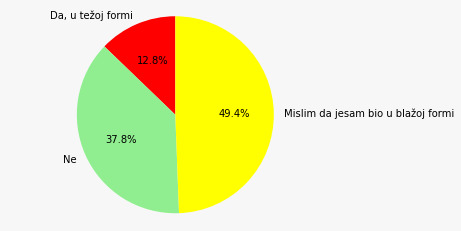
\includegraphics[width=\linewidth]{procenat_ljudi_doziveli_mobing.jpeg}
        \caption{Prikaz \% osoba koje su doživele mobing}
        \label{slika1}
    \end{figure}
    
    Globalno, mobing takođe predstavlja veliki problem, čemu svedoči podatak da je tokom svog radnog veka čak 17,9\% zaposlenih muškaraca i žena izjavilo da je bilo izloženo psihološkom nasilju na poslu u nekom trenutku, prema podacima koje je iznela Organizacija ujedinjenih nacija \cite{unreport}. U istraživanju sprovedenom 2021. je pronađeno da je čak 79\% zaposlenih u nekom trenutku bilo svedok ili žrtva nekog od oblika mobinga, a 66\% je bilo i samo podvrgnuto mobingu \cite{wpeareport}. Prema istom istraživanju, najčešći moberi su kolege, tj. zaposleni na istoj lestvici u kompanijskoj hijerarhiji (52\%), a tek zatim nadređeni (direktni nadređeni - 33\%, eksterni menadžeri - 8\%), dok ostali zaposleni čine najmanju frakciju mobera (6\%).
    
    \section{Primeri mobinga}
    
    \subsection{Slučaj Majkla Mersike}
    
    Pred Teksaškim sudom je 2014. godine pokrenut postupak od strane Majkla Mersike protiv kompanije \textit{Microsoft} koji se tiče mobinga. Majkl je u to vreme imao 47 godina, i bio jedan od istaknutih zaposlenih u kompaniji. Naime, on je, nekoliko godina ranije, raskinuo sa ženom iz iste kompanije koja je, nakon raskida, napredovala i eventualno postala njegov menadžer. Jedna od Majklovih koleginica ga je nakon toga optužila za seksualno zlostavljanje (što je jedna od stavki koje spadaju u mobing) i prijavila ga Majklovoj bivšoj devojci. Majkl je nakon toga doživljavao raznovrsne oblike ličnog deradiranja i poteškoća na poslu: smanjivan mu je budžet, bio je sprečavan da dobija povišice i unapređenja i td. On se takođe žalio \acrshort{hr} odeljenju zbog ponašanja njegove bivše partnerke i ostalih menadžera (koji su bili na njenoj strani), ali se ispostavilo da su ti napori bili uzaludni \cite{mercieca1}.
    
    Nakon ovoga g. Mersika je uložio žalbu nadležnom sudu i, nakon 4 godina borbe i preko 90 hiljada preglednih dokumenata, sa dva advokata na njegovoj strani i 250 advokata na strani njegovog protivnika, kompanije \textit{Microsoft}, uspeo je da pobedi. Isprva mu je porota dodelila 11,6 milliona američkih dolara, ali je sudija nadležan za slučaj tu sumu preinačio na dva miliona. Kako jedan od njegovih advokata, Pol Morin, navodi, \quotes{umesto da urade pravu stvar, menadžment je nasrnuo na Mersiku optužujući ga za seksualno napastvovanje i sveteći mu se} \cite{mercieca2}.
    
    \subsection{Grupni mobing u Guglu}
    
    Juna 2017. godine, tehnički gigant \textit{Gugl} izgubio je klasni spor pred kalifornijskim Vrhovnim sudom u San Francisku \cite{ellisgoogle}. Kako se u tužbi navodi, Gugl je vršio polnu diskriminaciju protiv svojih zaposlenih ženskog pola (navodi se da je, kao deo klasne tužbe, protiv Gugla učestvovalo oko 15.500 zaposlenih žena), plaćajući ih manje za slične poslove koji su obavljale od svojih muških kolega. Proces je trajao skoro 4 godine (od septembra 2013.), i tužbom je bilo pokriveno 236 pozicija na kojima su oštećene žene radile. Ovaj sudski postupak, osim što će dodeliti novčana sredstva oštećenim ženama, ima potencijal da naredi Guglu da vrši reviziju svojih \acrshort{hr} praksi vezanih za azpošljavanje od strane trećih lica. Holi Piz, jedna od imenovanih u tužbi, navela je da je zavodovoljna ishodom suđenja i da se, kao neko ko je svoj čitav radni ver proveo u \acrshort{it} stefi, nada da će ovo biti tačka počev od koje će jednakost žena i muškaraca u Guglu i industriji biti sve izraženija \cite{juristgoogle}.
    
    \subsection{Primeri mobinga u IT industriji u Srbiji}
    Iako je i u Srbiji prisutan mobing u IT sektoru, gotovo da nema slučajeva sa sudskim epilogom ili da su dospeli u javnost. Razlozi za to su što žrtve mobinga najčešće nađu drugi posao ili promene tim u kratkom roku. Kompanije kojima je delatnost outsourcing ostvaruju profit kroz razliku cene sata koju naplaćuju klijentima i cene sata koju isplaćuju zaposlenom. U takvim kompanijama postoji veliki rizik od mobinga koji ima za cilj držanje niskih plata radi povećanja profita. Takav mobing je često sistemski usmeren na sve zaposlene. Navešću nekoliko primera kojima sam ili prisustvovao ili poznajem žrtve.
    \begin{itemize}
        \item Zaposlenima, koji se ne osećaju dobro, skrenuta je pažnja da ne treba da uzimaju slobodan dan, ako ne moraju, i da to prijavljuju klijentu, nego da probaju da usporenim tempom izguraju radno vreme. Podstiče se kvazi junačenje u tom smislu, a zaposleni koji se ne uklapaju u takozvani junački profil, često bivaju predmet šale.
        \item Često menadžeri komentarišu zdravstveno stanje zaposlenog i sugerišu da idu na preglede van radnog vremena jer, po njihovoj proceni stanje nije hitno i nije vredno odricanja od naplativih sati.
        \item Podstiče se simultan rad na više projekata paralelno koji se naplaćuje u celosti od klijenata i povremeno lažiranje radnih sati koji su utrošeni na određenom zadatku kako bi se ostvarila korist od drugog projekta na kojem je zaposleni radio. Zaposleni koji ne pristaju na ovakve aktivnosti po pravilu imaju ograničen napredak u kompaniji i često su žrtve mobinga od strane nadređenih.
    \end{itemize}
    Ima dosta ovakvih primera, a svi oni imaju za cilj da povećaju broj naplativih sati i da poslodavac ostvari višestruku korist od jednog zaposlenog. U takvoj kompetitivnoj atmosferi, lako je postati žrtva mobinga ukoliko se ne uklapate u profil idealnog zaposlenog.
    
    
    \section{Zaključak}
    Mobing je u ljudskoj istoriji prisutan oduvek. Može se shvatiti kao neki vid zlostavljanja ljudi zaposlenih u istom ili, na neki način povezanom, preduzeću, i to na način koji uzrokuje individuu da se oseti ugroženom, i, potencijalno, napusti posao. Mobing je svetski opšteprisutan (više od 60\% zaposlenih je bilo žrtva mobinga u nekom obliku). Postoje različite vrste mobinga, i on se uglavnom razvija kroz nekoliko osnovnih faza -- počevši od manjih sukoba, on se razvija preko formi koje manifestuju psihološke simptome kod pojedinca, da bi eventualno rezultirao isključenjem s posla. Posledice ovakvog ponašanja, osim što utiču na radni koletiv u kompanijama, mogu da variraju -- od stresa pa sve do teških psihičkih i fizičkih posledica, a, u nekim slučajevima, i samoubistva.
    Međutim, postoje i mehanizmi koji omogućavaju pojedincima, pa čak i skupinama pojedinaca, da spreče, odnosno stanu na kraj zlostavljanju na radnom mestu. U ovim procesima je najuobičajenije i najprirodnije rešenje uključivanje hijerarhije nadređenosti tj. menadžmenta, kako bi se intervenisalo unutar same kompanije. Ipak, postoje i drugi oblici rešavanja mobinga, kao što su obraćanja posebnim društvima, agencijama ili na samom kraju sudovima.
    
    \glsadd{hr}\glsadd{it}
    \printnoidxglossary[type=\acronymtype,title=Skraćenice]
    
    \addcontentsline{toc}{section}{Literatura}
    \appendix
    \bibliographystyle{plain}
    \bibliography{literatura}
\end{document}
